%------------------------------------------------------------------------------
% physor2016_template.tex - template to write a contribution for the PHYSOR 
% 2016 conference
% v2.2 20151020 Wilfred van Rooijen, University of Fukui
%      Updated version to reflect the new style, without headers / footers.
% v2.1 20150717 Wilfred van Rooijen, University of Fukui
%      Extended template to illustrate more options with respect to figures and
%      references
% v2.0 20150508 Wilfred van Rooijen, University of Fukui
%      Created version for PHYSOR2016 meeting (Sun Valley)
% v1.0 20130422 Wilfred van Rooijen, University of Fukui
%      Created template for PHYSOR2014 meeting (Kyoto)
%------------------------------------------------------------------------------
% Usage: this template file should be used ONLY with pdfLaTeX. Place this 
%        template file and the file physor2016.sty in the your working
%        directory. If you use bibtex, put physor2016.bst and physor2016.bib 
%        also in the working directory. If you have your own BiBTeX database
%        file, make a copy or link in your working directory and replace 
%        \bibliography{physor2014} with \bibliography{your_bib_file}.
%
% NOTE: when compiling your document, you may get warnings regarding
%       the versions of several of the style files used in the PHYSOR2016 tem-
%       plate. A warning is issued if the version on your computer is older than
%       the version requested in the style file. Under normal circumstances, 
%       there should be no problems but when in doubt, please check the log file
%       and update your LaTeX distribution if necessary. 
%------------------------------------------------------------------------------
\documentclass[12pt]{article}
%
% NOTE: use \documentclass[12pt,draft]{article} for your initial work. This 
%       will give you the "draft" mode:
%       - a black marker is printed for each "overfull hbox" (*)
%       - figures are not included (only the BoundingBox is indicated)
%       - hyperref is switched off
%
% (*) In LaTeX, the text is typeset on the paper per paragraph - this is quite
%     different from MS Word where the text is typeset line-by-line. TeX will 
%     try to find an "optimal" layout of the paragraph. TeX uses "penalties" for
%     situations which are not optimal. TeX keeps re-setting the paragraph until 
%     the total penalty is minimized. To make an optimal layout, TeX uses line
%     breaking (hyphenation) and "spacing". For example, TeX can increase or de-
%     crease the space between words to fill out a line; in fact, TeX even 
%     allows to change the spacing between letters in a word - this is called
%     "kerning".
%     To make an optimal page layout, the line spacing is variable, and also
%     the spacing between paragraphs. In TeX vocabulary, these spaces are known
%     as "rubber lengths".
%     But sometimes TeX gets confused. For example, if you use very long words
%     and TeX cannot determine the proper hyphenation, of if you have an 
%     "inline" math section (an expression between $...$). In that case, 
%     there is no proper hyphenation. If the word is not too long, TeX will keep
%     the word on the line, but there will be "too many words" on the line; this
%     is known as "overfull hbox", and the last word will protrude into the 
%     right margin.  
%     If the word is really long, TeX will move the word to the next line, but
%     then the previous line will have "not enough words"; this is known as
%     "underfull". 
%     Both overfull and underfull boxes are not very satisfactory. TeX prints
%     the warnings into the log file. If the "draft" mode is on, then there 
%     will be a visible reminder in the PDF file of overfull and underfull 
%     boxes.
%
%     To prevent underfull / overfull boxes, basically you need to give TeX more
%     "options" to properly fill the line: 

%     - add hyphenation locations in long words: hy\-phe\-na\-tion
%     - rewrite the sentence so that the long word or the equation is not at
%       the end of the line
%     Try to get rid of all the underfull and overfull boxes - but sometimes a
%     it just can't be avoided. 
%
\usepackage{physor2016}
%
% The basic style file loads a minimum of other style files. If you need special 
% styles, simply include them here.
% !!! NOTE: the "amsmath" stylefile is included automatically by the physor2016 
% style file and thus you do not need to \usepackage{amsmath} !!!
%
% For real, bold face mathematical symbols
%
\usepackage{bm}
%
% To include figures in your paper. Note the following: manuscripts must be
% prepared in PDF. To do this, use pdflatex to produce PDF directly. pdflatex
% can include figures in the following formats: PDF, JPG, and PNG. For bitmap-
% ped images (photos etc), JPG is the preferred format, because JPG images can 
% be compressed very well in PDF, giving very small PDF files. For graphs and 
% schematics, vector images should be used; these can be either PostScript or
% PDF. If you have your figures as (e)ps, then see the notes at the end of this
% file for how to convert (e)ps to pdf. Note: bitmapped images should have
% a resolution of at least 300x300 dpi. For example, if your image has a size 
% of 1200x900 pixels, it should occupy not more than 4"x3" (approx 10x7.5 cm)
% in the manuscript. If you have many, large sized bitmap images which are 
% included with small size in the manuscript, then consider to re-size the 
% images before inclusion to maintain a reasonable size of the final PDF file.
%
% Making PDF images with Excel: use the Microsoft "save as PDF" plugin in 
% MS Office, and use the options of this plugin to export only one figure from
% you Excel file.
%
% To make very pretty diagrams etc with LaTeX, check out PGF/TikZ
%
\usepackage{graphicx}
\usepackage{tikz}
\usepgflibrary{shapes.geometric}
\usepackage{booktabs}
\usepackage{siunitx}
%
% If you use a table, check out this package. It creates tables with a little
% bit more space around the table entries. The result is a table that is easier
% to read, especially if you have mathematical super/subscripts in your work.
% Also check the manual of the package booktabs because it has some good tips 
% on how to make beautiful and informative tables.
%
\usepackage{booktabs}
%
% The following package takes care of setting SI units. Simply type 
% \degreeCelsius instead of $^\circ$ C. Also takes care of exponents and powers 
% of ten, as well as lining out numbers on the decimal point if required
\usepackage{siunitx}

\usepackage{epstopdf}
\usepackage{subcaption}
\usepackage{bigints}
\usepackage[section]{placeins}

%  new definitions
\newcommand{\bs}[1]{\mathbf{#1}}
\renewcommand{\div}{\bs{\nabla}\! \cdot \!}
\newcommand{\grad}{\bs{\nabla}}
% extra space
\newcommand{\qq}{\quad\quad}
% common reference commands
\newcommand{\eqt}[1]{Eq.~(\ref{#1})}                     % equation
\newcommand{\fig}[1]{Fig.~\ref{#1}}                      % figure
\newcommand{\tbl}[1]{Table~\ref{#1}}                     % table
\newcommand{\sct}[1]{Section~\ref{#1}}                   % section
\newcommand{\app}[1]{Appendix~\ref{#1}}                   % appendix

\newcommand{\keff}{k_\textit{eff}}

\newcommand{\be}{\begin{equation}}
\newcommand{\ee}{\end{equation}}
\newcommand{\vn}{\vec{n}}
\newcommand{\vel}{\vec{\mathrm{v}}}
\newcommand{\adj}{\Phi^\dagger_0}
\newcommand{\tcr}[1]{\textcolor{red}{#1}}

%------------------------------------------------------------------------------

%------------------------------------------------------------------------------
% Define title. Use all CAPITALS.
%------------------------------------------------------------------------------
\title{IMPLEMENTATION OF THE IMPROVED QUASI-STATIC METHOD IN RATTLESNAKE/MOOSE FOR TIME-DEPENDENT RADIATION TRANSPORT MODELLING}
%
% ...and authors
%
\author{ 
  \textbf{Zachary M. Prince and Jean C. Ragusa} \\
  Department of Nuclear Engineering \\
  Texas A\&M University, College Station, TX, USA\\
  \href{mailto:zachmprince@tamu.edu}{zachmprince@tamu.edu}\\
  \href{mailto:jean.ragusa@tamu.edu}{jean.ragusa@tamu.edu}\\
  \\                       % Put an extra empty line for different affiliations 
  \textbf{Yaqi Wang} \\
   Idaho National Laboratory \\
  \href{mailto:yaqi.wang@inl.gov}{yaqi.wang@inl.gov} 
}

%------------------------------------------------------------------------------
% The \shortauthor is printed on top of the even pages, and the \shorttitle
% is printed on top of the odd pages.
% Suggested format:
% - One author             : A. Author
% - Two authors            : A. Author \& B. Author
% - Three authors          : A. Author, B. Author \& C. Author
% - More than three authors: A. Author~et~al.
% If the title of your manuscript is very long, then make a short title such
% that it fits on one line in the header of the odd pages.
%
% NOTE: ANS requested that all headers / footers be removed from the template,
% and as a result, the author's names and paper title do NOT appear in the final
% document. However, the \shortauthor and \shorttitle are still used to set the
% PDF meta info in the PDF document, so please set these parameters to sensi-
% ble values.
%------------------------------------------------------------------------------
\renewcommand{\shortauthor}      % Author's names here
           {Prince {\em et. al.}}  
\renewcommand{\shorttitle}       % Short title here
           {IQS in Rattlesnake}

%------------------------------------------------------------------------------
% Setup PDF info. This sets several values which are listed as the "properties"
% of the PDF file.
%------------------------------------------------------------------------------
\hypersetup{
  pdftitle=\shorttitle,
  pdfauthor=\shortauthor
}

%------------------------------------------------------------------------------
% Begin document
%
% \doublespacing -- This option will increase the line spacing, making it 
%                   easier to add written comments etc. Be sure to switch it 
%                   off when you make the final version!
%
% \linenumbers -- switches on line numbers, which are practical when reviewing 
%                 a manuscript. Switch off line numbers when you make your 
%                 final version. 
%------------------------------------------------------------------------------
\begin{document}

%\doublespacing

%\linenumbers

%------------------------------------------------------------------------------
% Make the titlepage and set the pagestyle to fancy throughout
%------------------------------------------------------------------------------
\maketitle

\begin{abstract}
Because of the recent interest in reactor transient modeling and the restart of the Transient Reactor (TREAT) Facility, there has been a need for more efficient, robust methods in computation frameworks.  This is the impetus of implementing the Improved Quasi-Static method (IQS) in the RATTLESNAKE/MOOSE framework.  IQS has implemented with CFEM diffusion by factorizing flux into time-dependent amplitude and spacial- and weakly time-dependent shape.  The shape evaluation is very similar to a flux diffusion solve and is computed at large (macro) time steps.  While the amplitude evaluation is a PRKE solve where the parameters are dependent on the shape and is computed at small (micro) time steps.  IQS has been tested with a custom one-dimensional example and the TWIGL ramp benchmark.  These examples prove it to be a viable and effective method for highly transient cases. More complex cases are intended to be applied to further test the method and its implementation.
\end{abstract}

\keywords{RATTLESNAKE, MOOSE, TREAT, transient, factorization}

%------------------------------------------------------------------------------
%
%------------------------------------------------------------------------------
\section{INTRODUCTION}
\label{sect::intro}

The anticipated restart of Transient Reactor Testing (TREAT) Facility at Idaho National Laboratory (INL) has brought significant attention and opportunity to transient modeling.  TREAT, which was operational from 1954 to 1994, was designed to test nuclear fuels by subjecting them to various degrees of neutron pulses, from minor transients to accident cases.  Neutron transient modeling has always been computationally expensive due to implicit time-stepping caused by the neutron velocity values. Even with the vast improvements in computing technology, straightforward discretization of neutron conservation equations remain computationally challenging for real-world cases.  Therefore, methods that improve on computational speed significantly, at minimal detriment to accuracy, are highly desired. The Department of Energy (DOE) and INL have invested a substantial effort in modeling and simulation for TREAT.  This paper presents an implementation of the improved quasi-static (IQS) method for time-dependent neutron transport and diffusion equations with the multiphysics framework MOOSE \cite{moose}, notably its radiation transport application, RATTLESNAKE.

The improved quasi-static (IQS) method is a spatial kinetics method that involves factorizing the flux solution into space- and time-dependent components \cite{Ott_1966,Dulla2008}.  These components are the flux amplitude and its shape. Amplitude is only time-dependent, while the shape is both space- and time-dependent.  However, the impetus of the method is the assumption that the shape is only weakly dependent on time; therefore, the shape may not require an update at the same frequency of the amplitude function, but only on macro-time steps. As opposed to other forms of quasi-static approximations, the IQS method is not an approximation; the shape is updated consistently.  The results of IQS may only differ from straightforward, temporal discretization because the time discretization truncation error in the shape increases with a larger time-step size. 

Implementing IQS to RATTLESNAKE in INL's MOOSE framework is an obvious endeavor to enable high-fidelity modeling of the TREAT facility. The rest of this summary will briefly describe the derivation of IQS (in the diffusion setting for brevity), its current application to RATTLESNAKE using the the MultiApp Picard iteration capabilities of MOOSE, and results from examples testing the method's viability and effectiveness.

%------------------------------------------------------------------------------
%
%------------------------------------------------------------------------------
\section{BACKGROUND}
\label{sect::background}

In this Section, we recall the equations for the IQS method, starting from the standard multigroup diffusion equations written below:
\begin{align}
\frac{1}{v^g} \frac{\partial \phi^g }{\partial t} =& \frac{\chi_p^g}{\keff} \sum_{g'=1}^G (1-\beta) \nu^{g'} \Sigma_f^{g'} \phi^{g'} -  \left( -\div D^g \grad  + \Sigma_r^g \right) \phi^g  \nonumber \\
&  + \sum_{g'\neq g}^G\Sigma_s^{g'\to g} \phi^{g'}  + \sum_{i=1}^I\chi_{d,i}^g\lambda_i C_i \ , \quad 1 \le g \le G 
\end{align}
\be
\frac{dC_i}{dt} = \frac{\beta_i}{k_{eff}}\sum_{g=1}^G\nu^{g} \Sigma_f^g \phi^{g} - \lambda_i C_i \ , \quad 1 \le i \le I 
\ee
with
\be
\beta = \sum_{i=1}^I \beta_{i} 
\ee
Factorization is an important step in the derivation of the IQS method. The factorization approach leads to a decomposition of the multigroup flux into the product of a time-dependent amplitude ($p$) and a space-/time-dependent multigroup shape ($\varphi$):
\be
\phi^g(\vec{r},t)=p(t)\varphi^g(\vec{r},t)
\ee
To obtain the amplitude equations, the multigroup equations are multiplied by a weighting function, typically the initial adjoint flux ($\phi^*$), and then integrated over phase-space.  For brevity, the inner product over space will be represented with parenthetical notation:
\be
\int_D\phi^{*g}(\vec{r})f^g(\vec{r})d^3r=\left(\phi^{*g},f^g\right)
\ee
In order to impose uniqueness of the factorization, one requires the following:
\be
\sum_{g=1}^G\left(\phi^{*g},\frac{1}{v^g}\varphi^g\right) = \textit{constant}
\ee
After some manipulation, the standard point reactor kinetics equations (PRKE) for the amplitude solution are obtained:
\be
\frac{dp}{dt}=\left[\frac{\rho-\bar{\beta}}{\Lambda}\right]p+\sum_{i=1}^I\bar{\lambda}_i\xi_i
\ee
\be
\frac{d\xi_i}{dt}=\frac{\bar{\beta}_i}{\Lambda}-\bar{\lambda}_i\xi_i \quad 1 \le i \le I 
\ee
Where the functional coefficients are calculated using the space-/time-dependent shape function as follows:
\be
\frac{\rho-\bar{\beta}}{\Lambda}=\frac{ \sum_{g=1}^G\left(\phi^{*g},\frac{\chi_p^g}{k_{eff}}(1-\beta)\sum_{g'=1}^G \nu^{g'} \Sigma_f^{g'}\varphi^{g'} + \sum_{g'\neq g}^G\Sigma_s^{g'\to g} \varphi^{g'} -\left( -\div D^g \grad  + \Sigma_r^g \right)\varphi^g\right)}{\sum_{g=1}^G\left(\phi^{*g},\frac{1}{v^g}\varphi^g\right)}
\label{eq:rmb}
\ee
\be
\frac{\bar{\beta}}{\Lambda}=\sum_{i=1}^I\frac{\bar{\beta}_i}{\Lambda}=\sum_{i=1}^I\frac{1}{k_{eff}}\frac{\sum_{g=1}^G(\phi^{*g}, \chi_{d,i}^g\beta_i\sum_{g'=1}^G\nu^{g'} \Sigma_f^{g' }\varphi^{g'})}{\sum_{g=1}^G\left(\phi^{*g},\frac{1}{v^g}\varphi^g\right)}
\label{eq:b}
\ee
\be
\bar{\lambda}_i=\frac{\sum_{g=1}^G(\phi^{*g},\chi_{d,i}^g\lambda_i C_i)}{\sum_{g=1}^G(\phi^{*g},\chi_{d,i}^gC_i)}
\label{eq:l}
\ee

Finally, the shape equations are solved for the shape. The shape equations are similar to the orignal diffusion equations:
\begin{align}
\frac{1}{v^g} \frac{\partial \varphi^g }{\partial t} =& \frac{\chi_p^g}{\keff} \sum_{g'=1}^G (1-\beta) \nu^{g'} \Sigma_f^{g'} \varphi^{g'} -  \left( -\div D^g \grad  + \Sigma_r^g + \frac{1}{v^g}\frac{1}{p}\frac{dp}{dt}\right) \varphi^g  \nonumber \\
&  + \sum_{g'\neq g}^G\Sigma_s^{g'\to g} \varphi^{g'}  + \frac{1}{p}\sum_{i=1}^I\chi_{d,i}^g\lambda_i C_i \ , \quad 1 \le g \le G 
\label{eq:shape}
\end{align}
However, the amplitude and shape equations form a system of coupled equations: the coefficients appearing in the PRKEs depend upon the shape solution while the shape equation has a kernel dependent on amplitude and its derivative.  Because solving for the shape can be expensive, especially in two or three dimensions, it is attractive to make the assumption that the shape is weakly time-dependent so the shape can be computed after a multitude of PRKE calculations which is the root of IQS.  This is depicted schematically in \fig{fig:IQS}:
%
\begin{figure}[h]
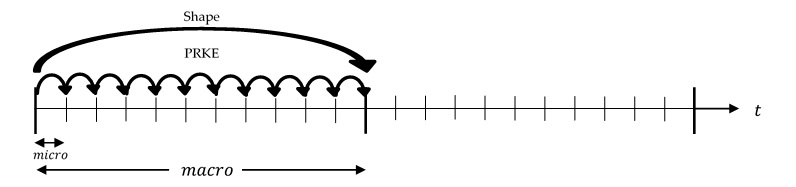
\includegraphics[width=\linewidth]{figures/IQS_visualization.jpg}
\caption{IQS method solution process}
\label{fig:IQS}
\end{figure}
%

Additionally, to improve consistency and accuracy, each macro time step can be iterated so the best shape is used to compute power at the micro time steps. Within the MOOSE framework,
nonlinear systems can be tackled in two manners: with Newton's method (usually, a preconditioned Jacobian-free version) and with Picard's iterations (fixed-point method). The latter is employed in the work. This iteration process must converge the shape such that the uniqueness condition $(\frac{d}{dt}\sum_{g=1}^G\left(\phi^{*g},\frac{1}{v^g}\varphi^g\right)=0)$ is preserved.

%------------------------------------------------------------------------------
%
%------------------------------------------------------------------------------
\section{IMPLEMENTATION IN RATTLESNAKE}
\label{sect::implementation}

MOOSE, or Multiphysics Object-Oriented Simulation Environment, is a finite-element-based  framework developed by INL and is equipped with advanced nonlinear solvers.  Rattlesnake is a module of MOOSE meant for neutronics and radiation transport problems.  RATTLESNAKE is a radiation transport application within MOOSE and can be coupled to other physics via a Newton or a Picard approach. Implementing the IQS in RATTLESNAKE is meant to enhance its transient modeling capability.  RATTLESNAKE utilizes an action system which initiates kernels, user objects, and postprocessors; these typically need to be added manually to the input file, but due to the large phase-space of neutron transport approximations, an automated action system is invoked to add the required MOOSE objects. When implementing the IQS, the action system and its associated MOOSE objects need to be updated. For brevity, we describe the implementation in the case of the CFEM Diffusion action system; similar developments are carried out for the DFEM Diffusion action system, the $S_n$ Transport action system, \ldots We discuss the CFEM Diffusion action system in detail: 

\begin{figure}[h]
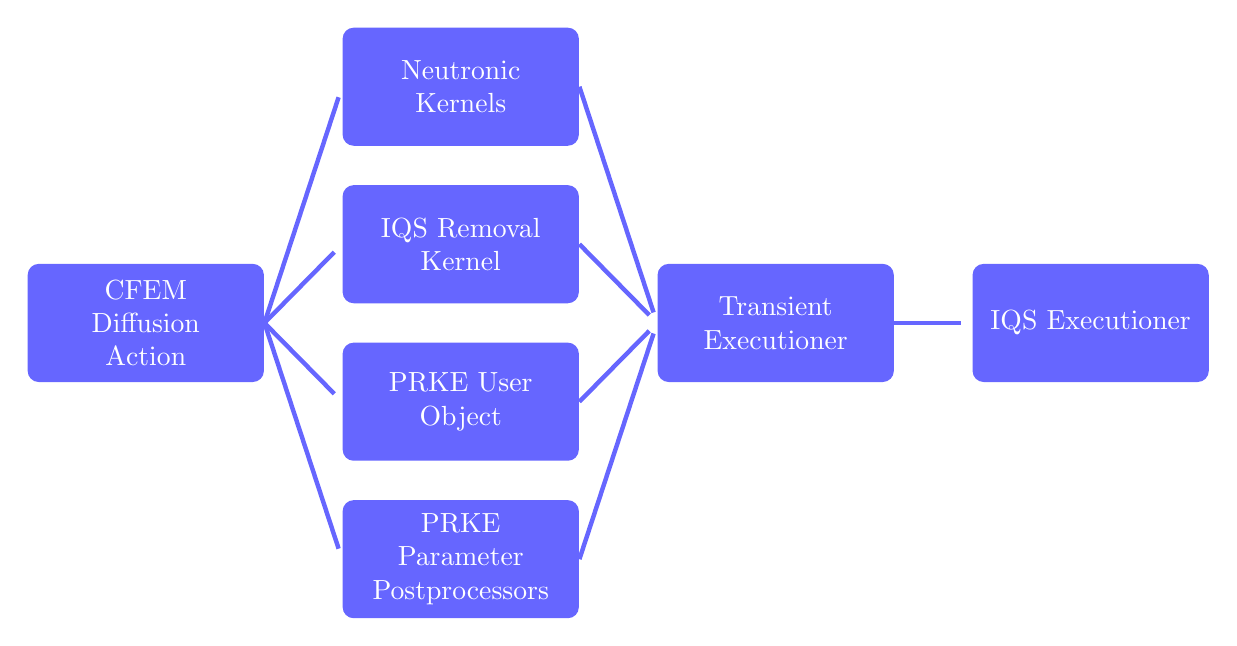
\begin{tikzpicture}[every node/.style = {shape          = rectangle, rounded corners, fill = blue!60, minimum width  = 3cm, minimum height = 1.5cm, align= center, text = white},blue edge/.style  = { -, ultra thick, blue!60, shorten >= 4pt}]
\node(0;0) at (0,0) {CFEM \\ Diffusion \\ Action};
  \node(1;3)  at (4, 3) {Neutronic \\ Kernels};   
  \node(1;1)  at (4, 1) {IQS Removal \\ Kernel}; 
  \node(1;-1)  at (4,-1) {PRKE User \\ Object}; 
  \node(1;-3) at (4,-3) {PRKE \\ Parameter \\ Postprocessors}; 
     \node(2;0)  at (8,0) {Transient \\ Executioner};
     	\node(3;0)  at (12,0) {IQS Executioner};
\foreach \j in {-3,-1,1,3}
  { \draw[blue edge] (0;0.east) -- (1;\j.west); }
\foreach \j in {-3,-1,1,3}
  { \draw[blue edge] (1;\j.east) -- (2;0.west);} 
\draw[blue edge] (2;0.east) -- (3;0.west);         
\end{tikzpicture}
\caption{CFEM Diffusion Action System Diagram}   
\label{Action}
\end{figure} 


%------------------------------------------------------------------------------
\subsection{Action System}

IQS derives its uniqueness from the executioner type; however, some additional changes needed to be carried out in the RATTLESNAKE/YAK action system in order to support IQS execution.   First, changes needed to be made in order to evaluate the shape equation.  The shape equation, after some manipulation, is very similar to the time-dependent flux equation, as seen in \eqt{eq:shape}.  To enable RATTLESNAKE to solve this shape equation in lieu of the standard diffusion equation, an additional removal kernel has to be instantiated to evaluate the quantity $\frac{1}{vp}\frac{dp}{dt}\varphi$ and added to FEM weak form  when the IQS executioner is selected.  Second, four postprocessors are created in order to calculate the PRKE parameters.  The parameter calculations were split into the following item: $\frac{\bar{\beta}_i}{\Lambda}$ numerator, $\bar{\lambda}_i$ numerator/denominator, $\frac{\rho}{\Lambda}/\frac{\bar{\beta}}{\Lambda}$ denominator, and $\frac{\rho-\bar{\beta}}{\Lambda}$ numerator.  The first three are relatively simple, only relying on material properties and solution quantities.  The $\frac{\rho-\bar{\beta}}{\Lambda}$ numerator requires the use of MOOSE's residual {\tt save\_in} feature, which saves the residual from a calculated kernel or boundary contribution in the shape evaluation to an auxiliary variable.  Finally, a user object was created to pull together all the postprocessor values and carryout the numerator/denominator divisions that were then passed to the executioner.

%%%%%%%%%%%%%%%%%%%%%%%%%%%%%%%%%%%%%%%%%%%%%%%%
\subsection{Precursor Integration}
%%%%%%%%%%%%%%%%%%%%%%%%%%%%%%%%%%%%%%%%%%%%%%%%
This section presents two different time-integration methods to solve coupled IQS shape + precursor equations, recalled below
using, for simplicity, a single neutron group and a single precursor group.

\be
\frac{1}{v}\frac{\partial\varphi}{\partial t}=\nu\Sigma_f(1-\beta)\varphi-\left(-\div D \grad + \Sigma_a + \frac{1}{v}\frac{1}{p}\frac{dp}{dt}\right)\varphi+\frac{1}{p}\lambda C 
\ee
\be
\frac{dC}{dt} = \beta\nu \Sigma_f \varphi p - \lambda C
\ee

First, we note that we could keep this system of two time-dependent equations and solve it as a coupled system. 
However, this is unnecessary and a memory expensive endeavor because the precursor equation is only an ODE and not a PDE. 
Instead, one may discretize in time the shape equation, which typically requires the knowledge of the
precursor concentrations at the end of the time step. This precursor value is taken from the solution, numerical or analytical,
of the precursors ODE. This document will discuss two techniques for solving the precursor equation.  First is a time discretization method that is currently being implemented in RATTLESNAKE.  The second is a analytical integration of the precursors, the latter method has proven to be more beneficial for IQS convergence.


\subsubsection{Time Discretization using the Theta Method}

A fairly simple way to evaluate the precursor equation is to employ the $\theta$-scheme ($0\le\theta\le1$),
explicit when $\theta=0$, implicit when $\theta=1$, and Crank-Nicholson when $\theta=1/2$).
Generally, if there is a function $u$ whose governing equation is $\frac{du}{dt}=f(u,t)$,
then the $\theta$-discretization is

\be
\frac{u^{n+1}-u^n}{\Delta t}=(1-\theta)f(u^n,t) + \theta f(u^{n+1},t) \,.
\ee

Applying this to the precursor equation:

\be
\frac{C^{n+1}-C^n}{\Delta t}=(1-\theta)\beta S_f^np^n-(1-\theta)\lambda C^n + \theta\beta S_f^{n+1}p^{n+1}-\theta\lambda C^{n+1}
\ee

Where $S_f$ is the fission source equivalent for shape:

\be
S_f^n=(\nu\Sigma_f)^n\varphi^n
\ee

Rearranging to solve for the precursor at the end of the time step yields

\be
C^{n+1} = \frac{1-(1-\theta)\Delta t\lambda}{1+\theta\Delta t\lambda}C^n + \frac{(1-\theta)\Delta t \beta}{1+\theta\Delta t\lambda}S_f^n p^n +  \frac{\theta\Delta t \beta}{1+\theta\Delta t\lambda}S_f^{n+1} p^{n+1}
\ee
Reporting this value of $C^{n+1}$, one can solve for the shape $\varphi^{n+1}$ as a function of $\varphi^n$ and $C^n$
(and $p^n$, $p^{n+1}$, $dp/dt|_n$ and  $dp/dt|_{n+1}$).
Once $\varphi^{n+1}$ has been determined, $C^{n+1}$ is updated. YAK currently implements both implicit and Crank-Nicholson as options for precursor evaluation.


\subsubsection{Analytical Integration}

Through prototyping, it has been found that neither implicit nor Crank-Nicholson time discretization of precursors are preferable methods for solving the shape equation in IQS.  It has been found that these discretizations result in a lack of convergence of the shape over the IQS iteration process.  In order to remedy the error, a analytical representation of the precursors was implemented in the prototype and the shape solution was able to converge (the normalization constant of the IQS method can be preserved to $10^{-10}$ while the theta-scheme only allowed convergence in the normalization factor to about $10^{-3}$).  The following section shows how this method was implemented in the prototype and RATTLESNAKE.

Using an exponential operator, the precursor equation can be analytically solved for:

\be
\int_{t_n}^{t_{n+1}} C(t')e^{\lambda t'} dt' = \int_{t_n}^{t_{n+1}} \beta(t') S_f(t') p(t')e^{\lambda t'}dt'
\ee

yielding

\be
C^{n+1} =  C^n e^{-\lambda (t_{n+1} - t_n) }  + \int_{t_n}^{t_{n+1}} \beta(t') S_f(t') p(t')e^{-\lambda (t_{n+1}-t')}dt'
\ee

Because $\beta$ and $S_f$ being integrated are not known continuously over the time step, they can be interpolated linearly over the macro step.  Such that:

\be
h(t) = \frac{t_{n+1}-t}{t_{n+1}-t_n}h^n  + \frac{t-t_n}{t_{n+1}-t_n}h^{n+1}  \quad t_n \le t \le t_{n+1}
\ee
% We let $\ell_n(t) = \frac{t_{n+1}-t}{t_{n+1}-t_n}$ and  $\ell_{n+1}(t) = \frac{t-t_n}{t_{n+1}-t_n}$ for simplicity. 

However, for the PRKE solve, we do have a very accurate representation of $p(t')$ over the time interval $[t_n,t_{n+1}]$.

Finally, we have the final expression for the analytical value for $C^{n+1}$:

\be
C^{n+1} = C^n e^{-\lambda \Delta t} 
+ \left(a_3\beta^{n+1}+a_2\beta^n\right)S_f^{n+1}
+ \left(a_2\beta^{n+1}+a_1\beta^n\right)S_f^n 
\ee

Where the integration coefficients are defined as:

\begin{align}
&a_1 = \int_{t_n}^{t_{n+1}}\left(\frac{t_{n+1}-t'}{\Delta t}\right)^2p(t')e^{-\lambda(t_{n+1}-t')}dt' \\
&a_2= \int_{t_n}^{t_{n+1}}\frac{(t'-t_n)(t_{n+1}-t')}{(\Delta t)^2}p(t')e^{-\lambda(t_{n+1}-t')}dt' \\
&a_3 = \int_{t_n}^{t_{n+1}}\left(\frac{t'-t_n}{\Delta t}\right)^2p(t')e^{-\lambda(t_{n+1}-t')}dt'
\end{align}

The amplitude $(p)$ is included in the integration coefficient because it has been highly accurately calculated in the micro step scheme, so a piecewise interpolation between those points can be done to maximize accuracy.  

The prototype code uses Matlab software to interpolate the amplitude between micro steps and a quadrature integration for the coefficients.  So the challenge for RATTLESNAKE was to replicate this procedure: passing the amplitude vector to the DNP auxkernel, interpolating it, and integrating the coefficients. 


%------------------------------------------------------------------------------
\subsection{Executioner}

The IQS executioner derives from the Transient executioner in MOOSE.  The IQS executioner contains a loop over micro time steps that solves the PRKEs and then passes the values for $p$ and $dp/dt$ at times corresponding to the macro-time steps into the Transient executioner in order to solve for the shape equation at each macro step.  The PRKEs are solved with two options, backward Euler and third order implicit Runge-Kutta method, within the Executioner.  The IQS executioner also supplements Transient's Picard iteration process by adding its own error criteria for the IQS method: 
\be
\text{Error}_{\text{IQS}}=\left|\frac{\left(\phi^*_g,\frac{1}{v_g}\varphi_g^n\right)}{\left(\phi_g^*,\frac{1}{v_g}\varphi_g^0\right)}-1\right|
\ee
The use of the Picard iteration capability of MOOSE's executioner will enable solving the nonlinear IQS equations along with other nonlinearly coupled multiphysics (e.g., thermal-hydraulics) using different time step sizes for neutronics and the other coupled physics. 


%------------------------------------------------------------------------------
%
%------------------------------------------------------------------------------
\section{RESULTS} 
\label{sect::results}

This section describes results of an examples that tests the IQS implementation and shows its effectiveness on computation speed and accuracy.  Two examples were selected for this purpose.  The first is a homogeneous one-group problem, subjected to a heterogenous material change (absorption cross-section change as a ramp in time for a subset of the geometry).  The second is the two-dimensional TWIGL ramp transient benchmark, described further.

%------------------------------------------------------------------------------
\subsection{One-Dimensional Custom Example}

The example is very simple and computes quickly, it entails a one dimensional, heterogeneous 400 cm slab with a varying absorption cross section.   Figure \ref{fig:slab} how the regions of the slab are divided and Table \ref{tab:1Dmat} shows the initial material properties.  Table \ref{tab:1Dslope} shows the ramp of the absorption cross-section of each region.

\begin{figure}[!htbp]
\begin{center}
\begin{tabular}{| l | l | l | l | l | l | l | l | l | l | l | l | l | l | l | l | l | l | l | l |}
\hline \hline \hline
  &   &   &   &   &   &    &    &   &   &   &   &   &   &   &   &   &   &   &   \\
  &   &   &   &   &   &    &    &   &   &   &   &   &   &   &   &   &   &   &   \\
1 & 1 & 1 & 1 & 2 & 3 & 1 & 1 & 1 & 1 & 1 & 1 & 1 & 1 & 4 & 4 & 1 & 1 & 1 & 1 \\
  &   &   &   &   &   &    &    &   &   &   &   &   &   &   &   &   &   &   &   \\
  &   &   &   &   &   &    &    &   &   &   &   &   &   &   &   &   &   &   &   \\
\hline \hline \hline
\end{tabular}
\caption{1-D heterogeneous slab region identification}
\label{fig:slab}
\end{center}
\end{figure}

\begin{table}[!htbp]
\begin{center}
\begin{tabular}{lllllll}
\toprule
Region & $D ()$ & $\Sigma_a (cm^{-1})$ & $\nu \Sigma_f (cm^{-1})$ & $v (cm/s)$ & $\beta$ & $\lambda (s^{-1})$ \\
\midrule
1 & 1.0 & 1.1 & 1.1 & 1,000 & 0.006 & 0.1 \\
2 & 1.0 & 1.1 & 1.1 & 1,000 & 0.006 & 0.1 \\
3 & 1.0 & 1.1 & 1.1 & 1,000 & 0.006 & 0.1 \\
4 & 1.0 & 1.1 & 1.1 & 1,000 & 0.006 & 0.1 \\
\bottomrule
\end{tabular}
\end{center}
\caption{1-D heterogeneous slab material properties and problem parameters}
\label{tab:1Dmat}
\end{table}

\begin{table}[!htbp]
\begin{center}
\begin{tabular}{lllllll}
\toprule
Material Property & 0.0 s & 0.1 s & 0.6 s & 1.0 s & 1.7 s \\
\midrule
$\Sigma_{a,2} (cm^{-1})$ & 1.1 & 1.1 & 1.095 & 1.095 & 1.095 \\
$\Sigma_{a,3} (cm^{-1})$ & 1.1 & 1.1 & 1.09 & 1.09 & 1.1 \\
$\Sigma_{a,4} (cm^{-1})$ & 1.1 & 1.1 & 1.105 & 1.105 & 1.105 \\
\bottomrule
\end{tabular}
\end{center}
\caption{1-D heterogeneous slab absorption cross-section slope perturbation}
\label{tab:1Dslope}
\end{table}



Figure~\ref{fig:power} shows the power at each macro time step as compared to the traditional brute force (full flux time discretization) method.  The strong correlation between the two curves shows that IQS is consistent with a proven method for a highly transient example.  Figure \ref{fig:conv} shows that IQS is not only consistent for this example, but also has a better error constant in the convergence study.  Figures \ref{fig:initial} - \ref{fig:final} plots shape changes in the IQS method, showing where the shape solution is necessary and a simple PRKE evaluation is inadequate.

\begin{figure}[!htbp]
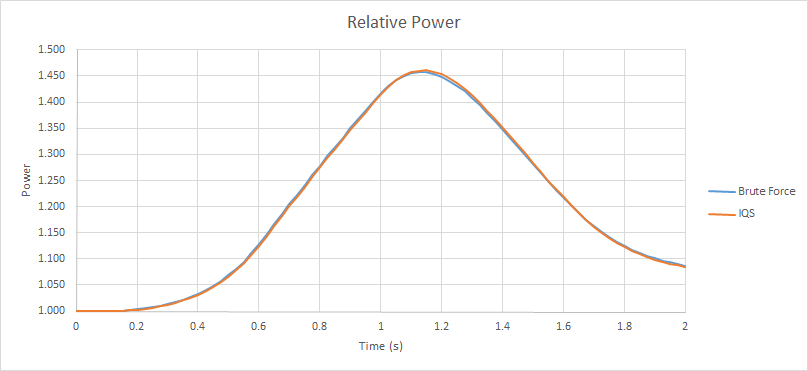
\includegraphics[width=\linewidth]{figures/1D_het_power_plot.png}
\caption{Power level comparison of 1D heterogeneous example between IQS and Brute Force using $\Delta t = 0.025$}
\label{fig:power}
\end{figure}

\begin{figure}[!htbp]
\begin{center}
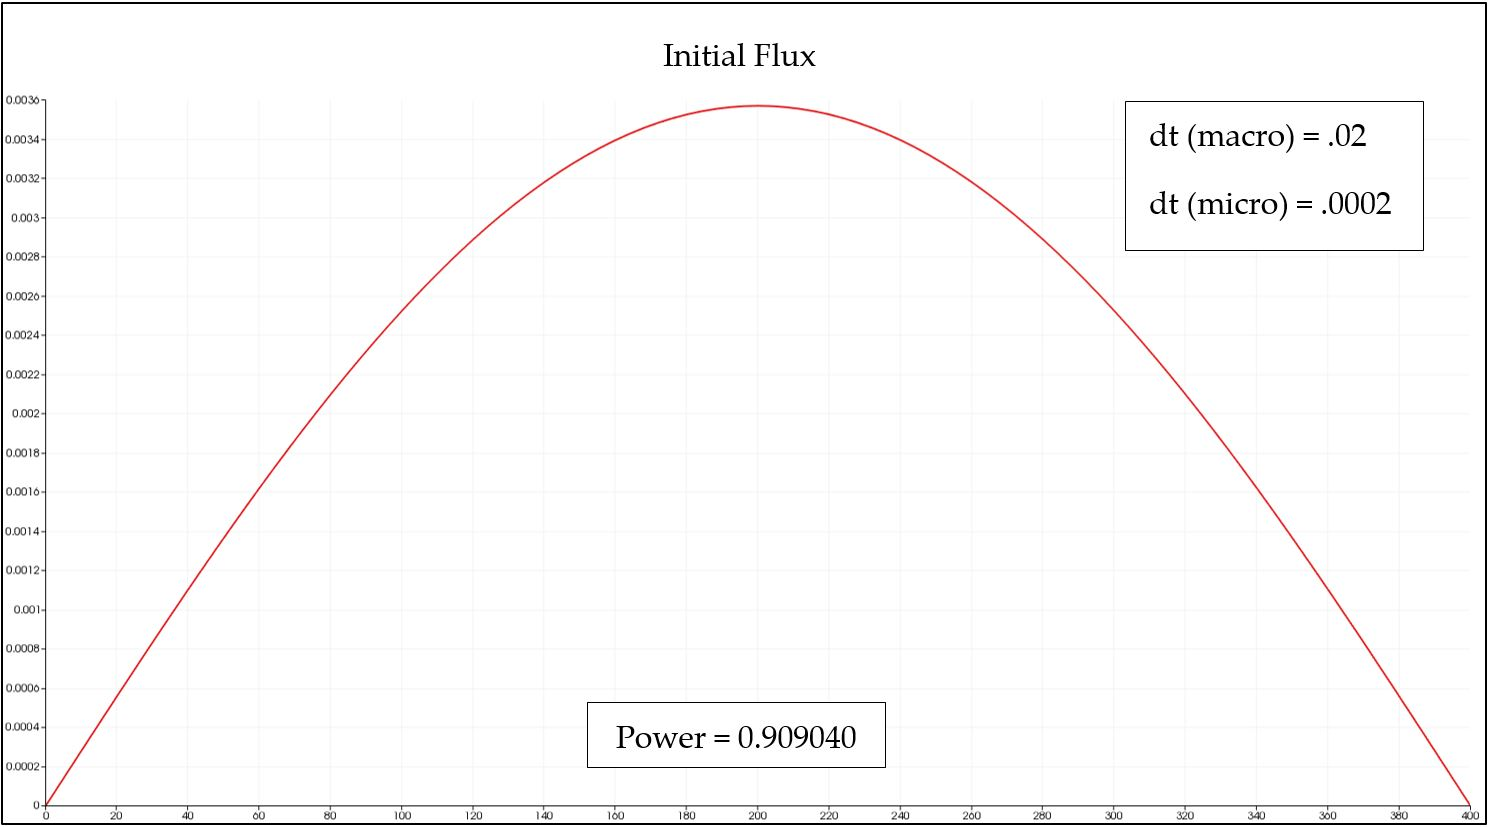
\includegraphics[width=5in,height=2in]{figures/initial_flux.jpg}
\caption{Initial Flux Plot}
\label{fig:initial}
\end{center}
\end{figure}

\begin{figure}[!htbp]
\begin{center}
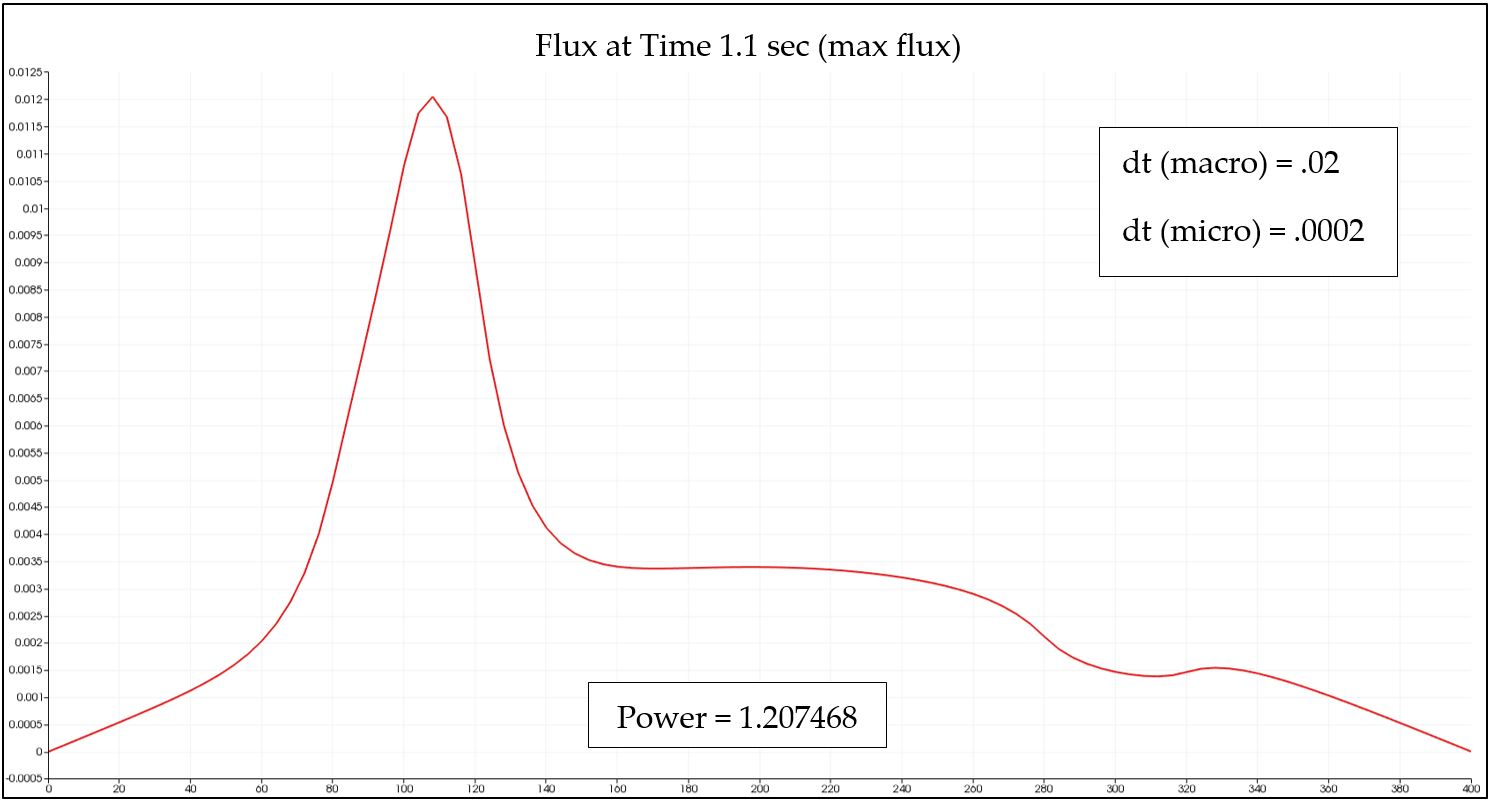
\includegraphics[width=5in,height=2in]{figures/max_flux.jpg}
\caption{Flux Plot when Absorption Cross Section is at Minimum}
\label{fig:max}
\end{center}
\end{figure}

\begin{figure}[!htbp]
\begin{center}
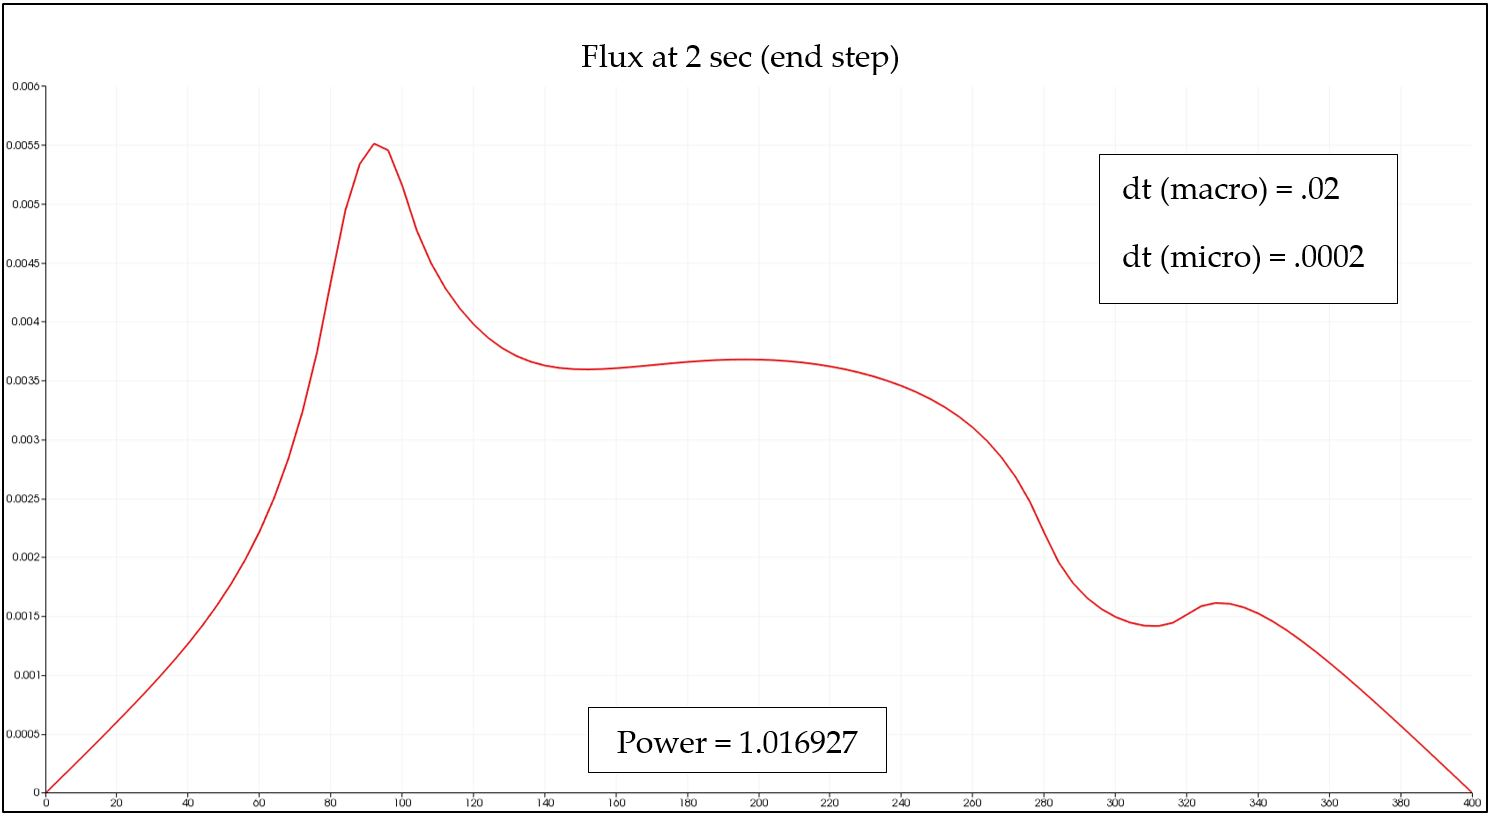
\includegraphics[width=5in,height=2in]{figures/final_flux.jpg}
\caption{Final Flux Computation (not steady-state)}
\label{fig:final}
\end{center}
\end{figure}

\begin{figure}[!htbp]
\centering
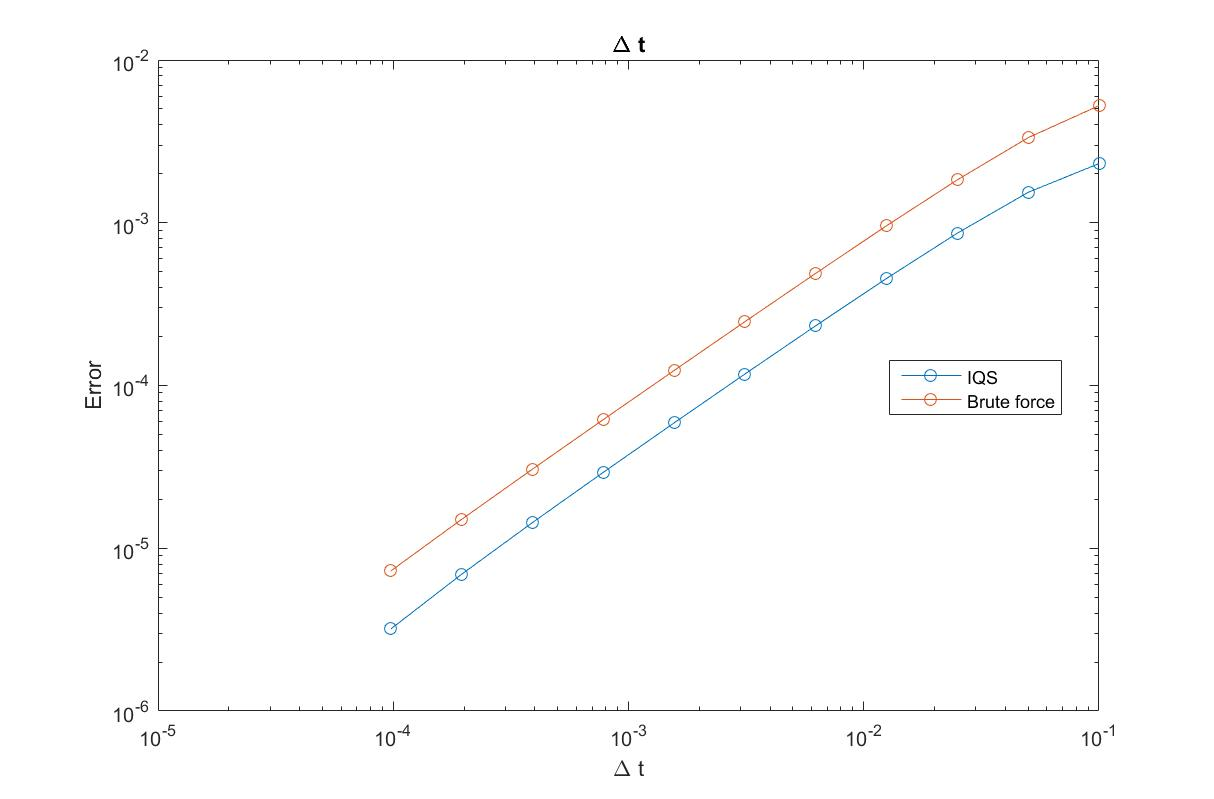
\includegraphics[width=4in]{figures/1D_het_convergence.jpg}
\caption{Error convergence comparison of 1D hetergenous example}
\label{fig:power}
\end{figure}

%------------------------------------------------------------------------------
\subsection{TWIGL Benchmark}

This benchmark problem originates from the Argonne National Lab Benchmark Problem Book.  It is a 2D, 2-group reactor core model with no reflector region shown in Figure \ref{fig:TWIGL_reg}.  Table \ref{tab:TWIGL_mat} shows the material properties of each fuel region and the ramp perturbation of Material 1.

\begin{figure}[!htbp]
\begin{center}
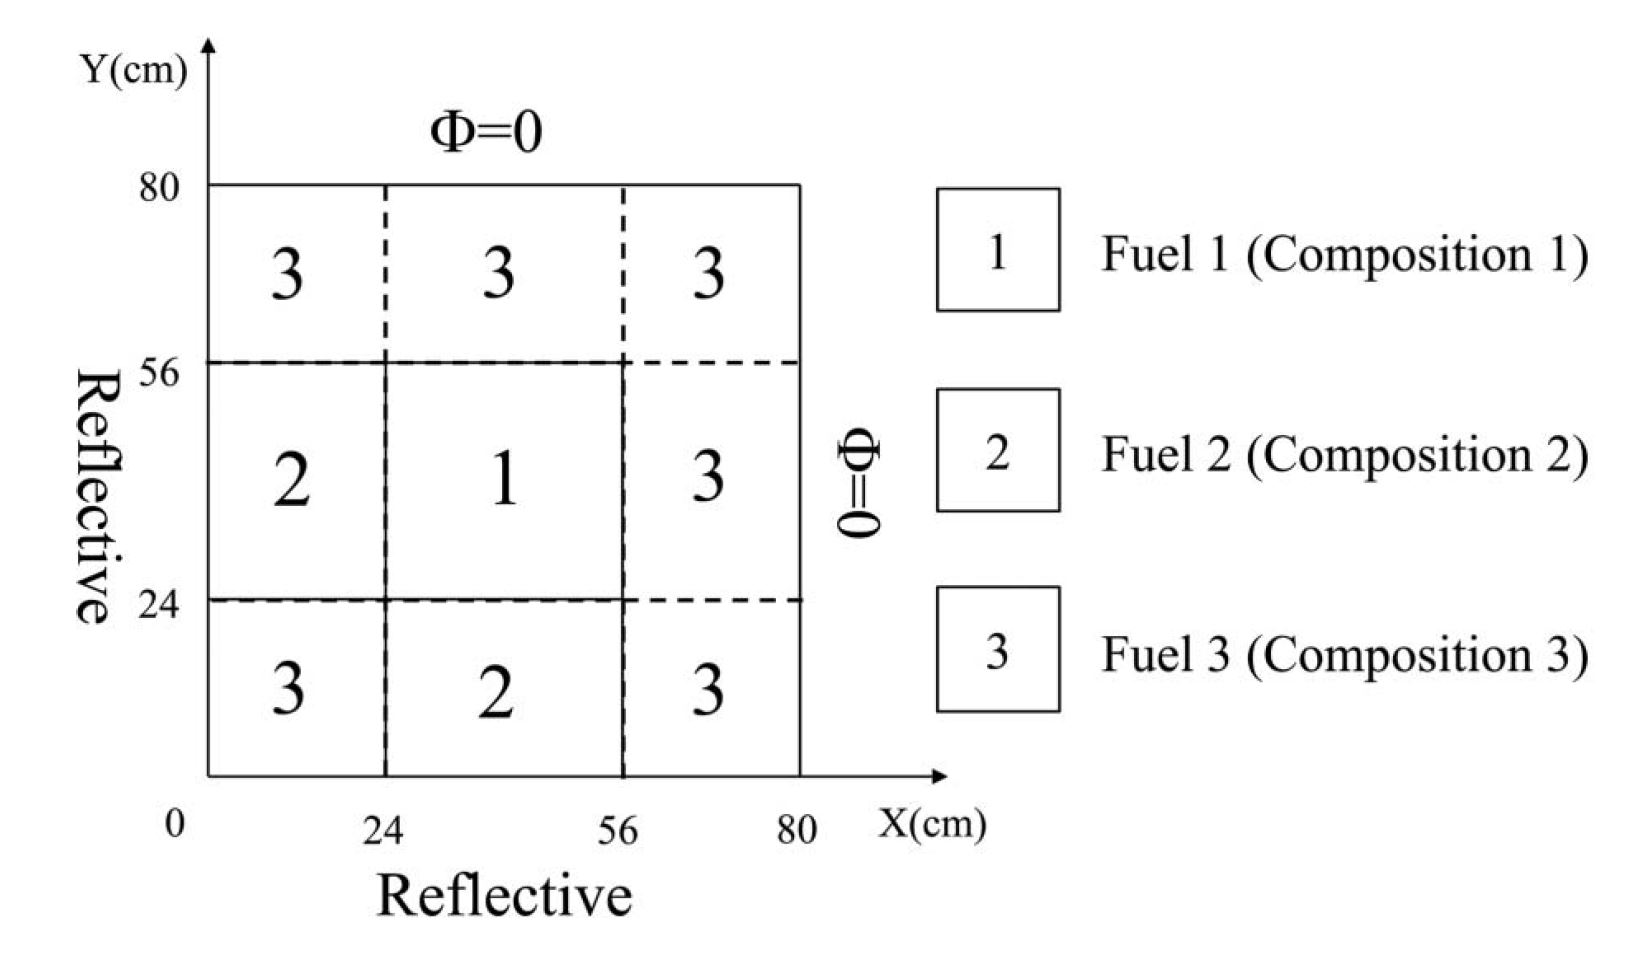
\includegraphics[width=4in]{figures/TWIGL_regions.jpg}
\caption{TWIGL benchmark problem description}
\label{fig:TWIGL_reg}
\end{center}
\end{figure}

\begin{table}[!htbp]
\begin{center}
\begin{tabular}{llllllll}
\toprule
  &  &  &  &  &  &  \multicolumn{2}{c}{$\underline{\Sigma_s (cm^{-1})} $} \\
Material & Group & $D (cm)$ & $\Sigma_a (cm^{-1})$ & $\nu\Sigma_f (cm^{-1})$ & $\chi$ & $g \rightarrow 1$ & $g \rightarrow 2$ \\
\midrule
1 & 1 & 1.4 & 0.010 & 0.007 & 1.0 & 0.0 & 0.01 \\
  & 2 & 0.4 & 0.150 & 0.200 & 0.0 & 0.0 & 0.00  \\
2 & 1 & 1.4 & 0.010 & 0.007 & 1.0 & 0.0 & 0.01  \\
  & 2 & 0.4 & 0.150 & 0.200 & 0.0 & 0.0 & 0.00  \\
3 & 1 & 1.3 & 0.008 & 0.003 & 1.0 & 0.0 & 0.01  \\
  & 2 & 0.5 & 0.050 & 0.060 & 0.0 & 0.0 & 0.00  \\
\midrule
  & $\nu$ & $v_1 (cm/s)$ & $v_2 (cm/s)$ & $\beta$ & $\lambda (1/s)$ &   &   \\
\midrule
  & 2.43 & 1.0E7 & 2.0E5 & 0.0075 & 0.08 &   &   \\
\bottomrule
 \multicolumn{8}{l}{\footnotesize Material 1 ramp perturbation:} \\
\multicolumn{8}{l}{\footnotesize $\Sigma_{a,2}(t)=\Sigma_{a,2}(0) \times (1-0.11667t) \quad t \leq 0.2 s$} \\
\multicolumn{8}{l}{\footnotesize $\Sigma_{a,2}(t)=\Sigma_{a,2}(0) \times (0.97666t) \quad t > 0.2 s$} \normalsize
\end{tabular}
\end{center}
\caption{1-D heterogeneous slab absorption cross-section slope perturbation}
\label{tab:TWIGL_mat}
\end{table}

Figures \ref{fig:TWIGL_power} and \ref{fig:TWIGL_plots} show the IQS  solution as compared with the Brute Force solution.  It is important to note the IQS shape plot is scaled differently than the Brute Force flux plot because the amplitude term is not included, but the gradients of colors is comparable.  These plots show that IQS is consistent in more complex, higher dimensional problems in RATTLESNAKE.  Finally, Figure \ref{fig:TWIGL_conv} plots the error convergence of IQS and the Brute Force methods.  The curves show the impressive convergence of IQS for the highly transience TWIGL example.

\begin{figure}[!htbp]
\centering
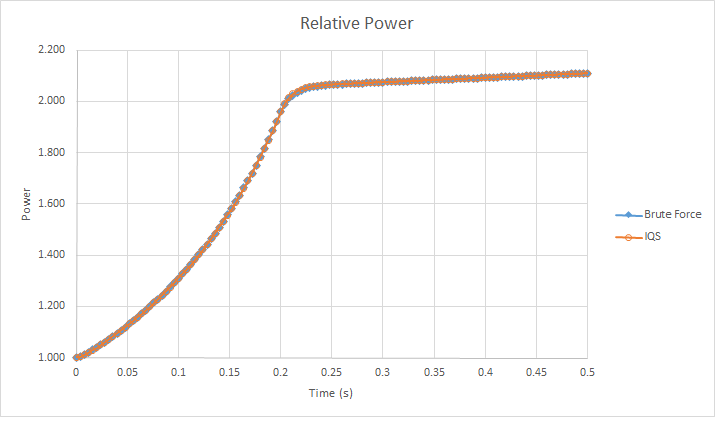
\includegraphics[height=3.0in]{figures/TWIGL_power_plot.png}
\caption{Power level comarison of 1D heterogeneous example between IQS and Brute Force using $\Delta t = 0.004$}
\label{fig:TWIGL_power}
\end{figure}

\begin{figure}[!htbp]
\begin{center}
\begin{subfigure}[!htbp]{0.4\textwidth}
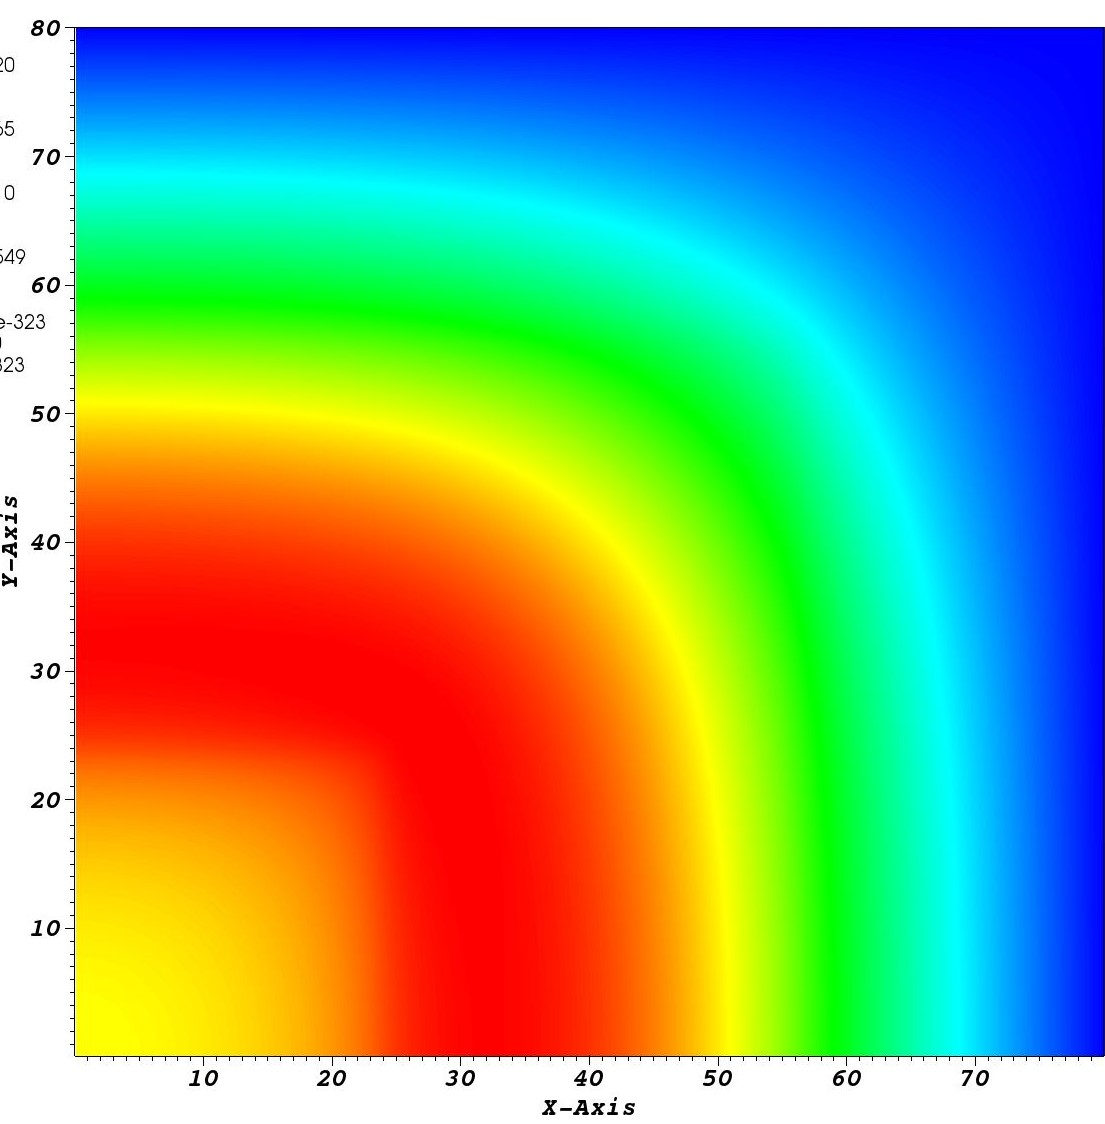
\includegraphics[width=\textwidth]{figures/ndiff_ramp_flux.jpg}
\caption{Brute force flux}
\end{subfigure}
\quad
\begin{subfigure}[!htbp]{0.4\textwidth}
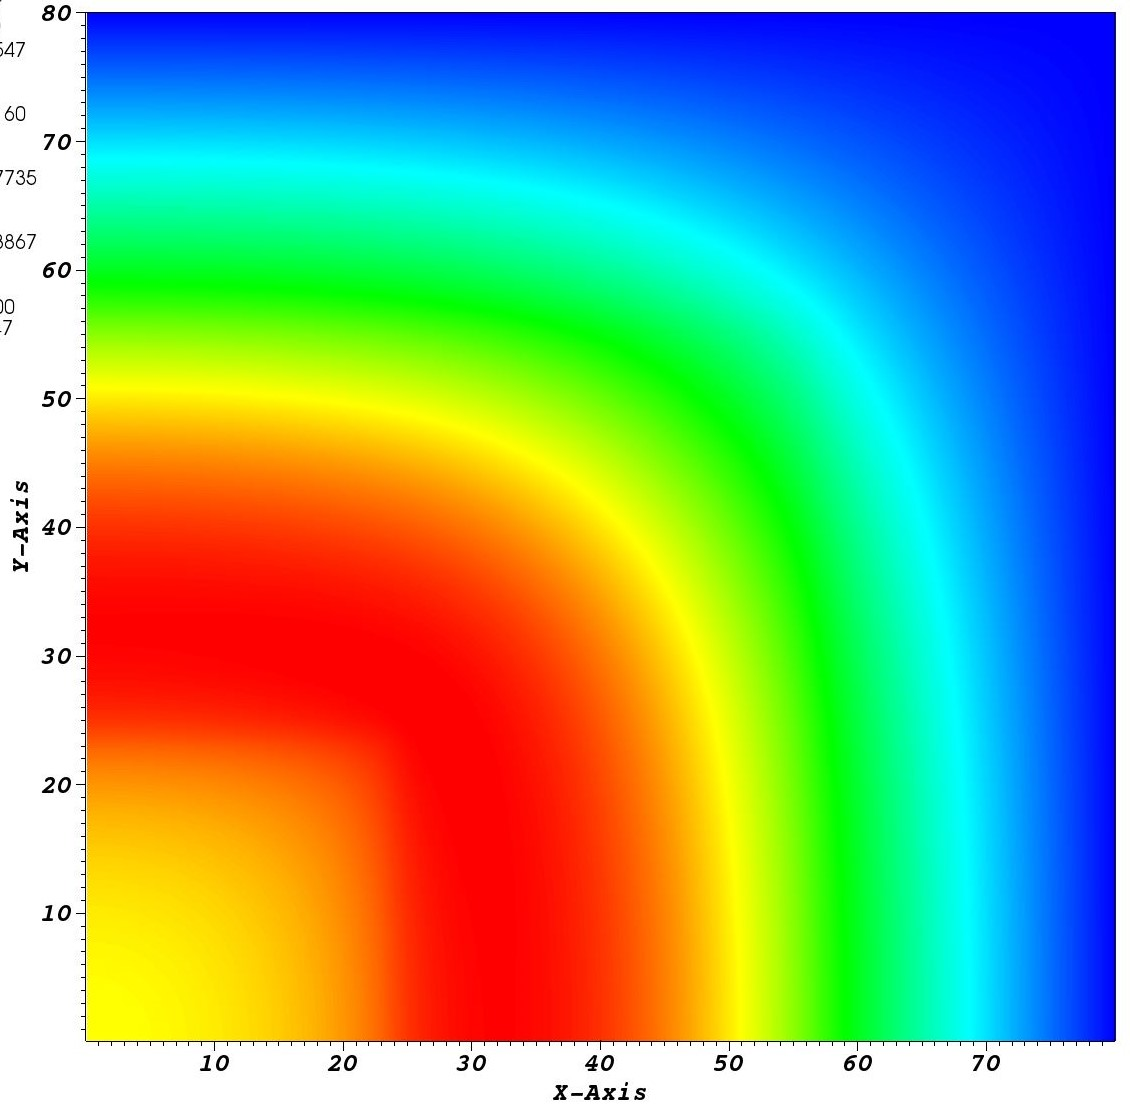
\includegraphics[width=\textwidth]{figures/iqs_ramp_shape.jpg}
\caption{IQS Shape}
\end{subfigure}
\caption{TWIGL Benchmark flux/shape comparison at $t=0.2$}
\label{fig:TWIGL_plots}
\end{center}
\end{figure}

\begin{figure}[!htbp]
\centering
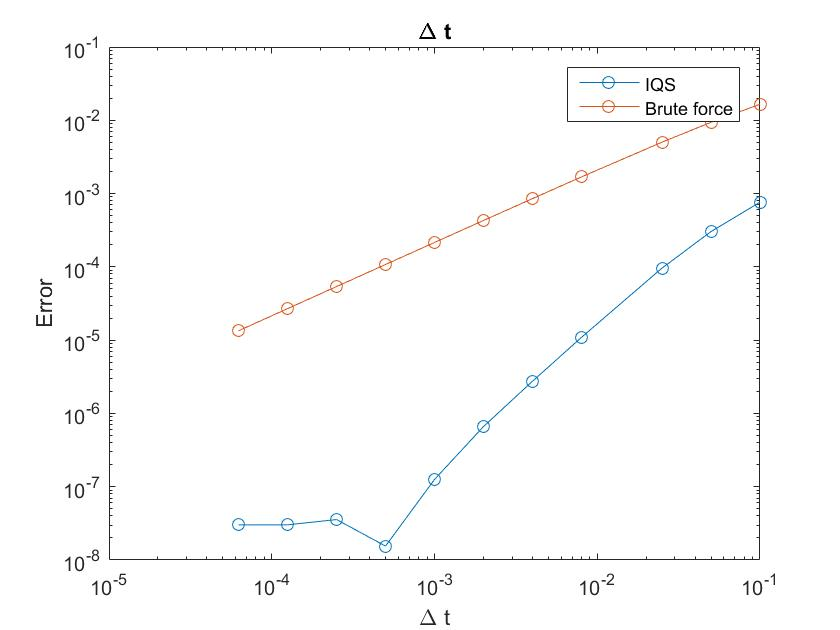
\includegraphics[width=4in]{figures/TWIGL_convergence.jpg}
\caption{Error convergence comparison of TWIGL Benchmark}
\label{fig:TWIGL_conv}
\end{figure}

%------------------------------------------------------------------------------
\section{Conclusions} 
\label{sect::ccl}

We have implemented the IQS method within RATTLESNAKE, part of the MOOSE framework. The implementation is complete for the CFEM Diffusion neutron equation and under testing for
DFEM Diffusion and $S_n$ transport equations. The application of IQS in MOOSE's Picard nonlinear solver was a relatively simple task using the object-oriented features of the framework. Once the implementation was completed for one action system, extension to other neutron discretizations is straightforward and elegant.  

The examples presented in this paper prove that IQS was not only a properly implemented in the MOOSE framework, but a incredibly effective method for highly transient cases.  More complex benchmarks (LRA and LMW benchmarks) and realistic cases (TREAT) are intended to be carried out using IQS (e.g., \cite{Yasinsky_1965, LMW_benchmark}), including a multiphysics neutronics+heat conduction reactor dynamic problem \cite{ANL_BPB}.

%------------------------------------------------------------------------------
%
%------------------------------------------------------------------------------
\bibliographystyle{physor2016}
\bibliography{references_IQS}



\end{document}


